\section{Compressione di Sorgente} \label{sec:sorg}
Il nostro obiettivo \`e quello di  associare  ad  ogni  simbolo informativo una sequenza di codice (di solito una sequenza binaria). Nel fare questo consideriamo sempre  una sorgente discreta di informazione, ovvero un  qualsiasi  elemento  del sistema  in  grado  di  produrre  una  successione  di  simboli  informativi ed  un canale ideale,  totalmente  affidabile, che quindi non altera l’informazione trasmessa (a ciascun simbolo inviato corrisponderà esattamente lo stesso simbolo ricevuto).
Di conseguenza l’operazione di decodifica ricostruirà esattamente i simboli della sorgente discreta originaria.
Esistono due tipi di codifiche di sorgente:
\begin{itemize}
    \item \textbf{Codifica lossy} (con perdita): si  applica  soprattutto  a  sorgenti  audio  e  video,  si  sfruttano fenomeni percettivi per    ridurre    la    quantità    di    bit    da    trasmettere. La cascata    dei processi di compressione/decompressione  porta  in  uscita  ad  un  flusso  digitale  diverso  da  quello in  ingresso. Tuttavia, si fa in modo che la perdita sia tollerabile (o addirittura irrilevante) per l’utente finale. La  compressione con perdite ha il vantaggio che può ottenere tassi di compressione molto più elevati rispetto a quella senza perdite.
    \item \textbf{Codifica lossless} (senza perdita): si  applica  \textit{solo  a  sorgenti  discrete} e  lo  scopo  della  codifica  di sorgente  è  quello  di  permettere  la  ricostruzione \textit{integrale} di  quanto  trasmesso,  che  dunque  viene detto senza perdita di informazione. La cascata dei processi di compressione/decompressione porta esattamente allo stesso flusso digitale che si ha in ingresso. 
\end{itemize}
Noi ci occuperemo della codifica lossless.
\subsection{Tipi di codice}
Un codice è una mappatura di una sequenza di simboli di una sorgente $S$ con alfabeto $X = \{x_1, \dots, x_n\}$ in una sequenza di simboli appartenenti  ad  un  altro  alfabeto $B = \{b_1, \dots, b_m\}$ di qualsiasi lunghezza.
\defn{\textit{Codice:}} Un codice \`e una funzione $C(\cdot)$ che associa ad ogni simbolo della sorgente una stringa di elementi appartenenti ad un alfabeto $B$:
\begin{equation}
    C: X \to B^*
\end{equation}
Dove $B^*$ rappresenta l'insieme di tutte le stringhe sull'alfabeto $B$. Dato un simbolo $x \in X$ la parola di codice (\textit{codeword}) associata si denota con $C(x)$.

Ovviamente non tutti i codici vanno bene, ce ne sono alcuni che sono preferibili, ed in particolare ciò che ci interessa di un codice è:
\begin{itemize}
    \item La \textbf{non ambiguit\`a}: ovvero la possibilità del ricevitore di ricostruire la successione di simboli 
trasmessi della sorgente S, senza ambiguità.
    \item L'\textbf{efficienza}: minore \`e la lunghezza media del codice utilizzato meglio è, dovendo trasmettere meno bit.
\end{itemize}
\defn{\textit{Lunghezza media:}} La lunghezza media di un codice, misurata in $[bit/simbolo]$ è definita come:
\begin{equation}
    L = \mathbb{E}_p[l(x)] = \sumx p(x)l(x)
\end{equation}
dove $l(x)$ \`e la lunghezza della parola di codice associata ad $x$. La media viene ovviamente fatta sulla distribuzione della sorgente. Vedremo in seguito come questa quantit\`a sia legata all'efficienza di un codice.\\
Oltre all’efficienza un codice  deve  garantire  la non  ambiguità: non  tutti  i  codici per\`o la garantiscono\footnote{Si pensi al caso banale in cui $X = \{a,b,c\}$ e $C(a)=C(b)=C(c)=0$: in ogni caso si riceve $0$ e non \`e possibile risalire al simbolo inviato.} e  quindi  dobbiamo  andare  a  considerare solo  il  sottoinsieme di codici per cui si verifica questa propriet\`a. L’ambiguità è data dalla possibilit\`a di associare la stessa parola di codice a due simboli diversi. Rendendo quindi necessaria l'imposizione che il codice sia una funzione iniettiva, si definiscono i \textbf{codici non-singolari}:
\defn{\textit{Codice non-singolare:}} Un codice viene detto non-singolare quando:
\begin{equation}
    \forall x_i, x_j \in X : x_i \neq x_j \implies C(x_i) \neq C(x_j)
\end{equation}
Tuttavia avere un codice non singolare non è sufficiente a garantire la non ambiguità, dovendo anche tenere in conto delle concatenazioni definiamo l'estensione $k$-esima del codice $C$:
\defn{\textit{Estensione $k$-esima del codice $C$: $C^k$}} \`E una funzione dall'insieme delle stringhe di $k$ simboli della sorgente all'insieme delle parole sull'alfabeto $B$, data dalla concatenazione delle singole parole di codice:
\begin{equation}
    C^k : X^k \to B^*, \quad C^k(x_1 x_2 \dots x_k) = C(x_1)C(x_2)\dots C(x_k)
\end{equation}
Quindi l’estensione $k$-esima del codice mappa una sequenza di $k$ simboli della sorgente $S$ in una sequenza di $k$ parole di codice.
\defn{\textit{Codice univocamente decodificabile (UD):}} Un codice si dice \textbf{univocamente decodificabile} se l’estensione $k$-esima del codice è non-singolare, per ogni valore di $k$.

È possibile verificare se un codice è univocamente decodificabile controllando “prefissi” e “suffissi”. Prendendo una generica parola di codice $C(x) = (b_1 b_2 \dots b_p)$ qualsiasi sequenza $(b_1 \dots b_k)$ di $k < p$ simboli \`e un \textit{prefisso} mentre la sequenza $(b_{k+1}\dots b_p)$ prende il nome di \textit{suffisso}.
La procedura per determinare se il codice \`e UD \`e la seguente: \\
Si prendono \textit{tutte le possibili coppie di parole di codice} e si controlla se qualcuna è il prefisso di un’altra. Nel caso si aggiunge il suffisso alle parole di codice. Si ripete fino a che:
\begin{itemize}
    \item Uno dei suffissi aggiunti è una parola di codice: Il codice \textbf{non \`e UD}.
    \item Non ci sono più suffissi da aggiungere: Il codice \textbf{\`e UD}.
\end{itemize}

\begin{mybox}{green}{\textit{\textbf{Esempio 1} : \textbf{Codici UD }}}
Vediamo due codici $C: \{a, b, c\} \to \{0, 1\}^*$
\begin{itemize}
    \item $C_1 = \{0, 01, 11\}$
    \begin{enumerate}
        \item $0$ \`e prefisso per $01$, dobbiamo quindi aggiungere il suffisso $\mathit{1}: C_1 = \{0,01,11,\mathit{1}\}$.
        \item $1$ \`e prefisso per $11$, dobbiamo quindi aggiungere il suffisso $\mathit{1}$, che \`e gi\`a presente.
        \item Non ci sono pi\`u suffissi da aggiungere quindi il codice \`e UD.
    \end{enumerate}
    \item $C_2 = \{0, 01, 10\}$
    \begin{enumerate}
        \item $0$ \`e prefisso per $01$, dobbiamo quindi aggiungere il suffisso $\mathit{1}: C_2 = \{0,01,10,\mathit{1}\}$.
        \item $1$ \`e prefisso per $10$, dobbiamo quindi aggiungere il suffisso $\mathit{0}: C_2 = \{0, 01, 10, \mathit{1}, \mathit{0}\}$.
        \item Il suffisso $\mathit{0}$ \`e uguale ad una parola di codice, quindi il codice non \`e UD.
    \end{enumerate}
\end{itemize}
\end{mybox}
C’è per\`o un’altra caratteristica che ci interessa, ovvero la velocità  di  decodifica. Esistono infatti codici non singolari e UD che però hanno il difetto che per poter rilevare quello che è stato trasmesso senza ambiguità richiedono di attendere la ricezione di un certo numero di simboli consecutivi. Questo \textit{introduce un ritardo di decodifica}. \\
Un codice si dice \textbf{istantaneo} (\textit{prefix-free}) se è possibile decodificare qualunque parola di codice della sequenza senza fare riferimento alle successive parole di codice. Esiste una condizione necessaria e sufficiente che esprime questa definizione:
\defn{\textit{Codice istantaneo:}} Un codice si dice istantaneo quando nessuna parola di codice è il prefisso di un'altra.
Nel  codice  istantaneo  nessuna  parola è prefisso di un’altra quindi  non  ci  sono suffissi  che  possono essere parole di codice (dal momento che non esistono suffissi).

\begin{minipage}{0.45\textwidth}
\begin{figure}[H]
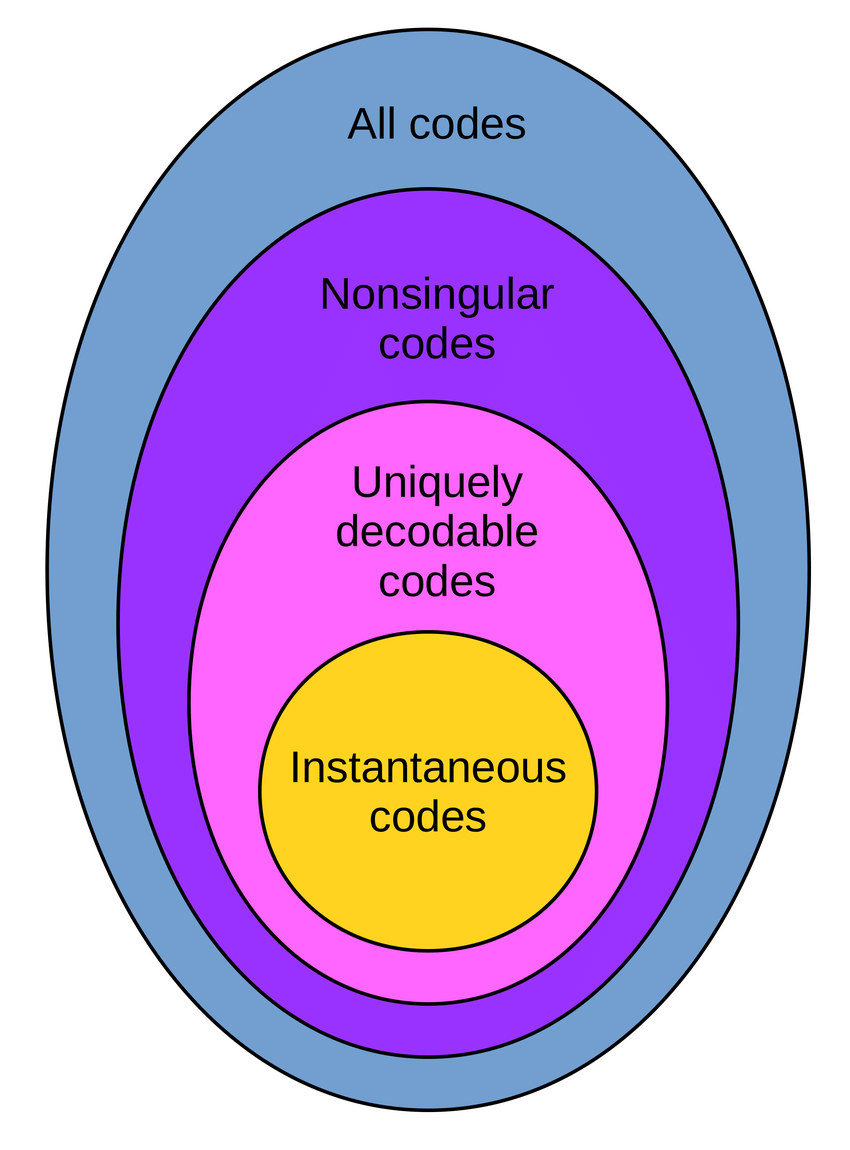
\includegraphics[scale=0.2]{img/codes.png}
\caption{\label{fig:codes} Gerarchia dei codici.}
\end{figure}
\end{minipage}
\begin{minipage}{0.45\textwidth}
Supponendo di avere una sorgente $S$ che emette simboli sull'alfabeto $X = \{a,b,c,d\}$ esaminiamo quattro codici $C: X \to \{0,1\}^*$ e le loro propriet\`a.
\begin{table}[H]
\begin{tabular}{l|l|l|l|l}
\toprule
$X$ & \textcolor{MidnightBlue}{Singolare} & \textcolor{RoyalPurple}{Non-singolare} & \textcolor{Lavender}{UD} & \textcolor{Dandelion}{Istantaneo} \\
\midrule
$a$ & 0         & 0             & 10  & 0          \\
$b$ & 0         & 010           & 00  & 10         \\
$c$ & 0         & 01            & 11  & 110        \\
$d$ & 0         & 10            & 110 & 111        \\
\midrule
    & $C_1$     & $C_2$         & $C_3$ & $C_4$ \\
\bottomrule
\end{tabular}
\label{tab:codici}
\end{table}
In particolare $C_3$ è UD ma non istantaneo perché non rispetta la regola del prefisso: se si riceve $11$ si deve aspettare i bit successivi per sapere se si è effettivamente ricevuto un $c$.
\end{minipage}

\subsection{Disuguaglianza di Kraft-McMillan}
Abbiamo detto che per la codifica di sorgente si è interessati solo ai codici istantanei, ma per ottenerli si devono rispettare  dei vincoli sulla lunghezza dei codici. Non è sempre possibile costruire codici UD e istantanei, ci sono delle condizioni che devono essere verificate. \\
Data una sorgente $S$ con alfabeto $X = \{x_1, x_2, \dots, x_N\}$ e un codice $C$ su un alfabeto\footnote{Nel caso in cui l'alfabeto di codifica sia binario $B = \{0,1\}$ e $|B|=R=2$.} $B = \{b_1, b_2, \dots, b_R\}$ che associa ad ogni simbolo $x_i$ un codice $C(x_i)$ di lunghezza $l_i = l(x_i)$ si ha una 

\textbf{Condizione Necessaria e Sufficiente} (\textbf{\textit{Disuguaglianza di Kraft-McMillan}}): \\
Affinch\`e esista un codice UD e istantaneo con parole di codice lunghe $l_1, l_2, \dots, l_N$ deve essere:
\begin{equation}
    \sum_{i=1}^N R^{-l_i} \leq 1
\end{equation}

Si vede  che  tale  disuguaglianza \textit{considera solo le lunghezze dei codici e niente  altro}. Inoltre, è importante sottolineare  che questo  teorema  dice  solo  che  \textit{se}  questa  condizione  è  soddisfatta sicuramente  \textit{esiste}  un codice univocamente  decodificabile ed istantaneo con queste lunghezze, ma \textit{non dice} che \textit{tutti} i codici con queste lunghezze  sono univocamente  decodificabili  ed istantanei, dice solo che  queste  lunghezze  sono corrette per costruire un univocamente decodificabile ed istantaneo.
\begin{tcolorbox}[enhanced, breakable, frame hidden]
\textbf{Dim}: \\
Dimostriamo prima la \textit{condizione sufficiente}, ovvero che, dati $R, l_1, l_2, \dots, l_N$:
\begin{equation*}
    \sum_{i=1}^N R^{-l_i} \leq 1 \implies \exists \text{ un codice istantaneo con queste lunghezze.}
\end{equation*}
Possiamo pensare, senza perdita di generalit\`a, di ordinare le lunghezze $l_i$ in ordine crescente e di chiamare $l$ la lunghezza massima $l \coloneqq \max \{l_1, l_2, \dots, l_N\}$ con $l > 0$. Quindi si avranno:
\begin{itemize}
    \item $n_1$ parole di codice lunghe $1$, con $n_1 \geq 0$.
    \item  $n_2$ parole di codice lunghe $2$, con $n_2 \geq 0$.
    \item $\dots$
    \item $n_{l-1}$ parole di codice lunghe $l-1$ con $n_{l-1} \geq 0$.
    \item $n_l$ parole di codice lunghe $l$, con $n_l > 0$.
\end{itemize}
Quindi possiamo riscrivere la disuguaglianza come:
\begin{equation*}
    \sum_{i=1}^N R^{-l_i} = \sum_{i=1}^{l} n_i R^{-i} \leq 1
\end{equation*}
Moltiplicando entrambi i membri per $R^l$ si ha che
\end{tcolorbox}
\begin{tcolorbox}[enhanced, breakable, frame hidden]
\begin{equation*}
    R^l \sum_{i=1}^{l} n_i R^{-i} = \sum_{i=1}^{l} n_i R^{l - i} \leq R^l
\end{equation*}
decomponendo la somma si ha
\begin{equation*}
    n_1 R^{l-1} + n_2 R^{l-2} + \dots +n_{l-2}R^2 + n_{l-1}R + n_l \leq R^l
\end{equation*}
isolando $n_l$ si ottiene
\begin{equation*}
    n_l \leq R^l - n_1 R^{l - 1} - n_2 R^{l - 2} - \dots - n_{l-1} R 
\end{equation*}
ma, essendo $n_l > 0$, anche 
\begin{equation*}
    0 < R^l - n_1 R^{l - 1} - n_2 R^{l - 2} - \dots - n_{l-1} R 
\end{equation*}
da cui
\begin{align*}
    &n_{l-1} R < R^l - n_1 R^{l - 1} - n_2 R^{l - 2} - \dots - n_{l-2}R^2 \\
    &n_{l-1} < R^{l-1} - n_1 R^{l-2} - n_2 R^{l -3} - \dots - n_{l-2}R
\end{align*}
Ricordando che $n_{l-1} \geq 0$ si ha
\begin{align*}
    &0 < R^{l-1} - n_1 R^{l-2} - n_2 R^{l-3} - \dots - n_{l-2}R \\
    &n_{l-2}R < R^{l-1} - n_1 R^{l-2} - n_2 R^{l-3} - \dots - n_{l-3}R^2 \\
    &n_{l-2} < R^{l-2} - n_1 R^{l-3} - n_2 R^{l-4} - \dots n_{l-3}R
\end{align*}
Proseguendo in questo modo fino a $n_1$ si ottiene
\begin{align*}
\begin{cases}
n_l \leq R^l - n_1 R^{l - 1} - n_2 R^{l - 2} - \dots - n_{l-1} R \\
n_{l-1} < R^{l-1} - n_1 R^{l-2} - n_2 R^{l -3} - \dots - n_{l-2}R \\
n_{l-2} < R^{l-2} - n_1 R^{l-3} - n_2 R^{l-4} - \dots n_{l-3}R \\
\dots \\
n_3 < R^3 - n_1 R^2 - n_2 R \\
n_2 < R^2 - n_1 R \\
n_1 < R
\end{cases}
\end{align*}
Quindi, ricapitolando, se vale la condizione di Kraft-McMillan sulle lunghezze $l_i$ si ha che valgono queste disequazioni, che altro non sono che la definizione alternativa di un codice istantaneo. \\
Dimostriamo ora la \textit{condizione necessaria}, ovvero che per un codice univocamente decodificabile (quindi anche per uno istantaneo$^{\ref{fig:codes}}$) con lunghezze $\{l_1, l_2, \dots, l_N\} \implies \sum_{i=1}^N R^{-l_i} \leq 1$. \\
Si ha
\begin{equation*}
    \Big ( \sum_{i=1}^N R^{-l_i} \Big )^n = \underbrace{\sum_{i=1}^N R^{-l_i} \sum_{j=1}^N R^{-l_j} \dots \sum_{k=1}^N R^{-l_k}}_n = \sum_{i=1}^N \sum_{j=1}^N \dots \sum_{k=1}^N R^{-(l_i + l_j + \dots + l_k)}
\end{equation*}
\end{tcolorbox}
\begin{tcolorbox}[enhanced, breakable, frame hidden]
Si ha che $p \coloneqq l_i + l_j + \dots l_k$ non \`e altro che la somma delle lunghezze di $n$ parole di codice. Chiamando come prima $l \coloneqq \max \{l_1, l_2, \dots, l_N\}$ si ha che $p \in [n, nl]$ (ovvero \`e compreso tra la somma di $n$ parole lunghe 1 ed $n$ parole lunghe $l$) da cui, chiamando $L_p$ il numero di concatenazioni di $n$ parole di codice le cui lunghezze sommate danno $p$, si ha:
\begin{equation*}
    \Big ( \sum_{i=1}^N R^{-l_i} \Big )^n = \sum_{i=1}^N \sum_{j=1}^N \dots \sum_{k=1}^N R^{-(l_i + l_j + \dots + l_k)} = \sum_{p=n}^{nl} L_p R^{-p}
\end{equation*}
Ma  la concatenazione  di $n$ parole di codice  non  è  altro  che la parola di codice  di  un  messaggio  di $n$ simboli, cio\`e  un  codice dell’estensione $n$-esima della sorgente $S^n$. Per definizione di univocamente decodificabile, quindi, qualunque sia l’estensione della sorgente ($\forall n$) si ha che presi due codici questi devono essere diversi. \\
Questo implica che, se abbiamo $L_p$ codici di lunghezza $p$, per fare in modo che siano diversi tra loro deve valere
\begin{equation*}
    L_p \leq R^p
\end{equation*}
Da cui:
\begin{align*}
    &\Big ( \sum_{i=1}^N R^{-l_i} \Big )^n = \sum_{p=n}^{nl} L_p R^{-p} \leq \sum_{p=n}^{nl} R^p R^{-p} = \sum_{p=n}^{nl} 1 = nl - n + 1  \leq nl
\end{align*}
quindi
\begin{equation*}
    \Big ( \sum_{i=1}^N R^{-l_i} \Big )^n \leq nl \implies \sum_{i=1}^N R^{-l_i} \leq 1
\end{equation*}
Infatti se fosse $ \sum_{i=1}^N R^{-l_i} > 1$ (quindi $\sum_{i=1}^N R^{-l_i} = 1 + \epsilon$) si avrebbe che, ad esempio
\begin{equation*}
\lim_{n \to \infty} \frac{(1+\epsilon)^n}{n} = \infty \nleq l
\end{equation*}

$\square$
\end{tcolorbox}

\subsection{Codici compatti}
Siamo adesso interessati a definire codici \textit{efficienti}. Iniziamo con una definizione:
\defn{\textit{Codice compatto:}} Un codice $\mathcal{C}$ si definisce compatto se: 
\begin{enumerate}
    \item \`E univocamente decodificabile.
    \item La sua lunghezza media $L_{\mathcal{C}}$ \`e la minore tra tutti gli altri codici UD per la sorgente $S$ sull'alfabeto $B$.
    \[
    L_{\mathcal{C}} \leq L_C, \quad \forall C: X \to B^*
    \]
\end{enumerate}
Per trovare codici compatti dobbiamo capire quale è la \textit{minima lunghezza possibile} di un codice. Assumendo momentaneamente che la sorgente $S$ sia una DMS (rilasseremo poi quest'ipotesi alle sorgenti di Markov) abbiamo un risultato molto importante. Si ha che, detta $H_b (S)$ l'entropia della sorgente $S$ in base $b$, 
\begin{equation}
    \frac{H(S)}{\log b} = H_b (S) \leq L
\end{equation}
ovvero che l'entropia della sorgente rappresenta un limite inferiore per la lunghezza media di un codice univocamente decodificabile. Questo  è  un  primo  importante  risultato  perché  \textit{lega  la  definizione  di  informazione/entropia  con  una quantità che non dipende dalla definizione stessa di informazione}.\\
Se, per un codice UD $\mathcal{C}$, vale il limite inferiore $H_b(S) = L_{\mathcal{C}}$ allora il codice \`e un \textbf{codice compatto}. Questo avviene quando $\forall x \in X, \exists l \in \mathbb{N}:$
%\begin{equation*}
%    H_b(S) = \sumx p(x) \log_b \frac{1}{p(x)} = \sumx p(x) l(x) = L_{\mathcal{C}} \implies \log_b  %\frac{1}{p(x)} = l(x) \implies  p(x) = b^{-l(x)}
%\end{equation*}
%cio\`e quando, 
\begin{equation*}
   p(x) = b^{-l}
\end{equation*}
nel caso in cui $b=2$ la sorgente si dice \textit{diadica}.
\begin{tcolorbox}[enhanced, breakable, frame hidden]
\textbf{Dim}: Dimostriamo che $H(S)-L \leq 0$, il caso generale non \`e molto diverso.
\begin{align*}
    H(S) - L &= \sumx p(x) \info{x} - \sumx p(x) l(x) = \\
    &= \sumx p(x) \info{x} - \sumx p(x) \log 2^{l(x)} = \\
    &= \sumx p(x) \log \frac{2^{-l(x)}}{p(x)} = \log e \sumx p(x) \ln \frac{2^{-l(x)}}{p(x)} \leq \\
    &\leq \log e \sumx p(x) \Big ( \frac{2^{-l(x)}}{p(x)} - 1 \Big ) = \\
    &=\log e \bigg ( \underbrace{\sumx 2^{-l(x)}}_{\leq 1} - \sumx p(x) \bigg ) \leq 0
\end{align*}
Inoltre l'uguaglianza vale quando le due disuguaglianze valgono con l'uguaglianza, cio\`e quando:
\begin{equation*}
\begin{cases}
\frac{2^{-l(x)}}{p(x)} = 1 \iff p(x) = 2^{-l(x)}, \hspace{5pt} \forall x \in X \\
\sumx 2^{-l(x)} = 1
\end{cases}
\end{equation*}
\hspace{400pt}$\square$
\end{tcolorbox}
Quindi, per una DMS in cui le probabilità di emissione siano della forma (generale), $\forall x \in X$
\begin{equation*}
    p(x) = b^{-l(x)} =  \Big ( \frac{1}{b} \Big )^{l(x)}
\end{equation*}
si può avere una lunghezza  di  codice  (istantaneo) \textit{minima pari all’entropia della  sorgente stessa}. Ovviamente  avere probabilità di questa forma non è realistico. Consideriamo allora il caso di una sorgente DMS in cui i valori di $p(x)$ siano arbitrari, quindi non rispettano nessun vincolo. Questo implica che $H_b(S) < L$, ovvero non si può più avere un codice di lunghezza minima possibile. 
\defn{\textit{Efficienza:}} Si definisce l'efficienza $\eta$ di un codice con lunghezza media $L$ per una sorgente $S$ come:
\begin{equation}
    \eta \coloneqq \frac{H_b(S)}{L}
\end{equation}
Quanto pi\`u questo numero (puro) si avvicina a $1$ tanto maggiore \`e l'efficienza della codifica. 
\subsection{Primo Teorema di Shannon}
Shannon ha  studiato  come  cercare  di  avvicinarsi  al  limite  minimo  anche  in  caso  in  cui le  probabilità  di emissione dei simboli siano arbitrarie. Ha pensato, nel caso in cui i valori di $p(x)$ siano arbitrari, di approssimare $l(x)$ con l’intero maggiore più vicino a quello di una sorgente diadica\footnote{In una sorgente diadica si ha, equivalentemente, $l(x) = \log_b p(x)^{-1}= -\log_b p(x)$}, cio\`e, $\forall x \in X$:
\begin{equation}
l_S(x) \coloneqq \bigg \lceil \log_b \frac{1}{p(x)} \bigg \rceil
\end{equation}
Si ha ovviamente che, $\forall x \in X$
\begin{equation}
    l(x) \leq l_S(x) \leq l(x) + 1
\end{equation}
e che il codice costruito con queste lunghezze \`e istantaneo, soddisfando la disugaglianza di Kraft-McMillan. Considerando infatti la prima delle due disugaglianze $l(x) \leq l_S(x)$ vale
\begin{align*}
    &l(x) = \log_b \frac{1}{p(x)} \leq l_S(x) \implies \frac{1}{p(x)} \leq b^{l_S(x)} \implies \\
    &\implies p(x) \geq b^{-l_S(x)} \implies \sumx p(x) = 1 \geq \sumx b^{-l_S(x)}
\end{align*}
Inoltre si ha che 
\begin{equation}
    H_b(S) \leq L \leq H_b(S) + 1
\end{equation}
\begin{tcolorbox}[enhanced, breakable, frame hidden]
\textbf{Dim}: Dimostriamo nel caso $b=2$. Si ha
\begin{align*}
    &\log \frac{1}{p(x)} \leq \hspace{2pt} l_S(x) \leq \info{x} + 1 \text{ da cui}\\
    &\underbrace{\sumx p(x) \info{x}}_{=H(S)} \leq \underbrace{\sumx p(x) l_S(x) }_{=L} \leq \sumx p(x) \Big ( \info{x} + 1 \Big ) = H(S) + 1 \\
    &\hspace{400pt}\square
\end{align*}
\end{tcolorbox}

\subsubsection{Sorgenti discrete senza memoria}
Shannon ha osservato che, estendendo la sorgente e codificando i messaggi invece dei singoli simboli la lunghezza media per codificare un simbolo si riduce.
Basandoci su questa osservazione si consideri la sorgente estesa $S^n$ in cui vengono inviati messaggi $\sigma_i$ di $n$ simboli appartenenti all'alfabeto $X = \{x_1, x_2, \dots, x_M\}$:
\begin{equation*}
    \sigma_i = \{ x_{i_1} x_{i_2} \dots x_{i_n} \}
\end{equation*}
Si hanno quindi $M^n$ possibili messaggi $\sigma$ emittibili dalla sorgente estesa $S^n$ caratterizzati da una probabilit\`a $p(\sigma)$. Scegliendo, seguendo la codifica di Shannon, un codice di lunghezza
\begin{equation}
    \lambda(\sigma) = \Big \lceil \log \frac{1}{p(\sigma)} \Big \rceil
\end{equation}
si ha, come prima
\begin{equation*}
   \log \frac{1}{p(\sigma)} \leq \lambda(\sigma) \leq \log \frac{1}{p(\sigma)} + 1
\end{equation*}
da cui, mediando su tutti gli $M^n$ messaggi $\sigma \in S^n$, si ottiene
\begin{equation}
    \sum_{\sigma \in S^n} p(\sigma) \log \frac{1}{p(\sigma)} \leq \sum_{\sigma \in S^n} p(\sigma) \lambda(\sigma) \leq \sum_{\sigma \in S^n} p(\sigma) \Big ( \log \frac{1}{p(\sigma)} + 1 \Big )
\end{equation} da cui
\begin{equation}
    H(S^n) \leq L_n \leq H(S^n) + 1
\end{equation}
in cui si \`e definito
\begin{equation}
    L_n \coloneqq \sum_{\sigma \in S^n} p(\sigma) \lambda(\sigma)
\end{equation}
ovvero la lunghezza media del codice per simbolo esteso (il numero medio di simboli dell’alfabeto di codice) quando si mandano e si decodificano $n$ simboli consecutivi.
Ricordando poi che $H(S^n) = nH(S)$ si ottiene
\begin{equation}
    H(S) \leq \frac{L_n}{n} \leq H(S) + \frac{1}{n}
\end{equation}
Si ha quindi che $L_n / n$, cio\`e il numero medio di simboli del codice usati per codificare un blocco di $n$ simboli, tende a $H(S)$ all'aumentare di $n$. \\
Si ha quindi il \textbf{Primo Teorema di Shannon per una DMS}: \textit{possiamo codificare una sorgente senza memoria con una lunghezza media per simbolo vicina a piacere al limite minimo (l'entropia della sorgente) codificando più simboli insieme invece che uno solo.} \\
Il prezzo che si paga è la complessità, dovendo codificare e decodificare $n$ simboli consecutivi lavorando con la sorgente estesa $S^n$.
\subsubsection{Sorgenti di Markov}
Sia ora $S$ una sorgente discreta con memoria di Markov. Quanto visto precedentemente per le sorgenti DMS in merito alla minima lunghezza di codifica vale anche per le sorgenti con memoria. Se infatti consideriamo $\bar{S}$, la sorgente aggiunta di $S$, essendo questa senza memoria vale quando già visto ovvero $H(\bar{S}) \leq L$. Ma vale anche $H(S) \leq H(\bar{S})$ da cui
\begin{equation}
    H(S) \leq L
\end{equation}
Possiamo estendere il Primo Teorema di Shannon alle sorgenti con memoria di Markov. \\
Per una sorgente di Markov $S$ di ordine 1 si ha
\begin{equation}
    H(S) + \frac{H(\bar{S}) - H(S)}{n} \leq \frac{L_n}{n} \leq H(S) + \frac{H(\bar{S}) - H(S)}{n} + 1
\end{equation}
mentre in generale per una sorgente di Markov di ordine $k$ vale, per un certo $\epsilon_k \in \mathbb{R}$
\begin{equation}
    H(S) + \frac{\epsilon_k}{n} \leq \frac{L_n}{n} \leq H(S) + \frac{\epsilon_k}{n} + 1
\end{equation}
\begin{tcolorbox}[enhanced, breakable, frame hidden]
\textbf{Dim}: Dimostriamo nel caso di una sorgente di Markov di ordine $1$. \\
Consideriamo l'aggiunta di $S$, ovvero la sorgente $\bar{S}$, si ha che, essendo questa una DMS, scelto $\forall x \in X$ un codice di Shannon dato da $l(x) = \lceil - \log p(x) \rceil$ (dove $p(x)$ \`e la probabilit\`a incondizionata), vale
\begin{equation*}
    H(\bar{S}) \leq L \leq H(\bar{S}) + 1
\end{equation*}
Si può quindi prendere la sorgente aggiunta $\overline{S^n}$ della sorgente estesa e arrivare esattamente come prima a scrivere
\begin{equation*}
    H(\overline{S^n}) \leq L_n \leq H(\overline{S^n}) + 1
\end{equation*}
Ricordando poi, dalla \ref{eqn:adjmarko}, che per una sorgente di Markov del primo ordine si ha
\begin{equation*}
    H(\overline{S^n}) = nH(S) + [H(\bar{S}) - H(S)]
\end{equation*}
da cui
\begin{equation*}
    H(S) + \frac{H(\bar{S}) - H(S)}{n} \leq \frac{L_n}{n} \leq H(S) + \frac{H(\bar{S}) - H(S)}{n} + 1
\end{equation*}
Per le sorgenti di Markov di ordine superiore l’espressione è analoga perché vale
\begin{equation*}
  \hspace{70pt}  H(\overline{S^n}) = nH(S) + \epsilon_k, \hspace{50pt} \square
\end{equation*}
\end{tcolorbox}